\documentclass[]{article}

\usepackage{listings}	
\usepackage{float}
\usepackage{graphicx}

\usepackage{titling}
\newcommand{\subtitle}[1]{%
  \posttitle{%
    \par\end{center}
    \begin{center}\large#1\end{center}
    \vskip0.5em}%
}

\begin{document}

\title{Lab 2}
\subtitle{CS M152A}
\author{Aman Agarwal \& Lowell Bander}

\maketitle
\tableofcontents \newpage

\section{Introduction}
\section{Design Description}

\subsection{High Level Design}
\label{subsec:highlevel}

To convert a value from its representation as a 12 bit two's-complement number to an 8 bit floating point number, we used 3 main modules. The first of which converted the input from a two's complement representation to a sign-magnitude representation. The second counts the number of leading zeros to determine the value of the exponent, and extracts the lower bits for use in determining the exponent. The third and final module handles the edge cases, such as rounding the significand and handling overflow.\\

Before we began implementing the converter in Verilog, we first drew up a schematic in Logisim, as pictured in Figure~\ref{fig:logisim}.\\

\begin{figure}[H]
\centering
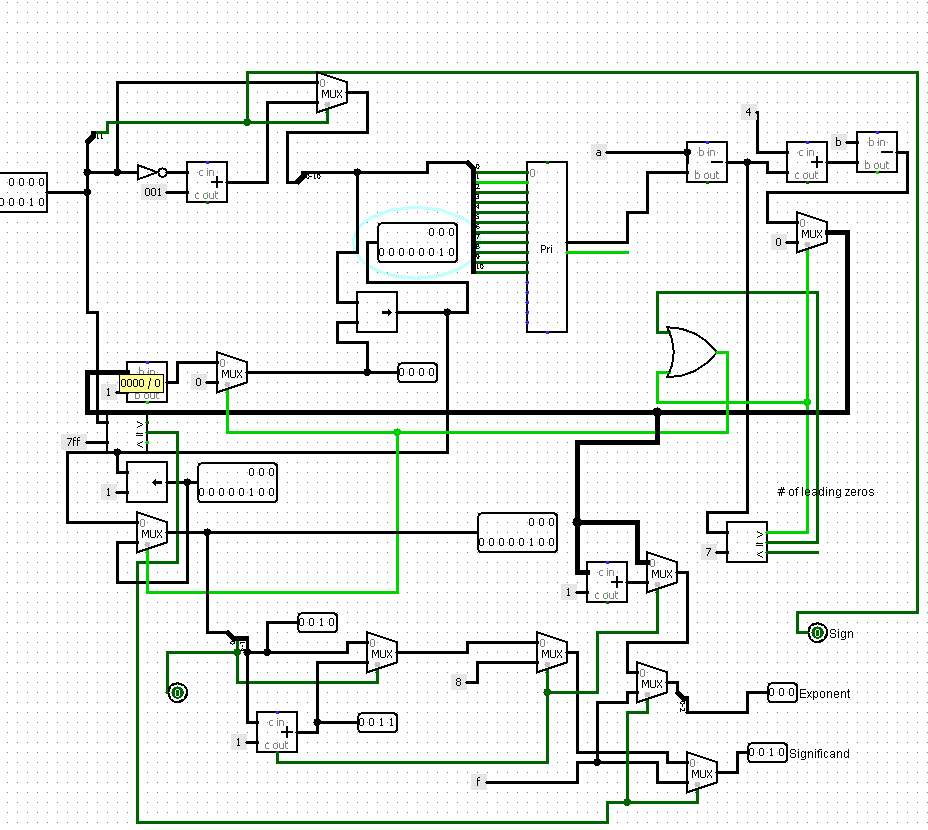
\includegraphics[width=11cm]{logisim.PNG}
\caption{A schematic for the converted drawn using Logisim. Input is delivered to the system in the upper-left, and output is found in the lower-right.}
\label{fig:logisim}
\end{figure}

\subsection{Low Level Implementation}

The source code displayed below is an a excerpt from our main module, \texttt{fpcvt.v}. The 3 modules described in subsection~\ref{subsec:highlevel} above are show here with the following mapping: The first module described above is composed of the first module shown below, which takes as input a 12 bit two's complement integer, and outputs an 8 bit sign-magnitude integer.\\

The next two modules have the same semantics as the second modules described above. The first modules, \texttt{leadingZeroesCount}, takes as input the magnitude of the input number, and outputs the number of leading zeros, for use later in determining the exponent. The following module, \texttt{extractSignificandAndRoundBit}, takes as input the magnitude of the input value and the number of leading zeros, and returns the 4-bit significand and the fifth bit used for rounding.\\

The final two modules below implement the 3rd module described above in subsection~\ref{subsec:highlevel}. The first of which, \texttt{roundValueIfRound}, takes as input the intermediate significand produced by the \texttt{extractSignificand\-AndRoundBit} module, as well as the fifth bit outputted by the the same module. The outputs of this modules are the rounded significand, if this was necessary, and a bit indicating whether overflow results from this rounding. The final module, \texttt{handleOverflow}, handles possible overflow by right shifting the significand and incrementing the exponent to account for this increment.

\begin{lstlisting}[frame=single, language=verilog, caption= Excerpt from main \texttt{fpcvt.v} module.]
twosComplementToSignMagnitude ttsm(.I(D), .S(S), .M(mag));
    
leadingZeroesCount lzc(.I(mag), .O(zeroCount));
    
extractSignicifandAndRoundBit esr(.I(mag), 
.zeros(zeroCount), .significand(tempF), .round(round));

roundValueIfRound rvir(.I(tempF), .roundedVal(rv), 
.Round(round), .overflow(overflow));

handleOverflow ho(.I(D), .roundedVal(rv), .significand(F), 
.oldE(tempE), .exponent(E), .overflow(overflow));
\end{lstlisting}



\section{Simulation Documentation}
\section{Conclusion}


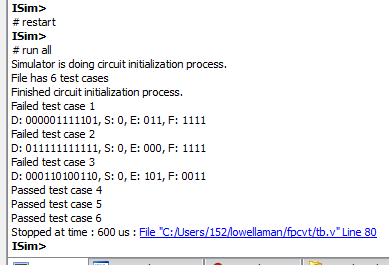
\includegraphics[width=10cm]{output.PNG}

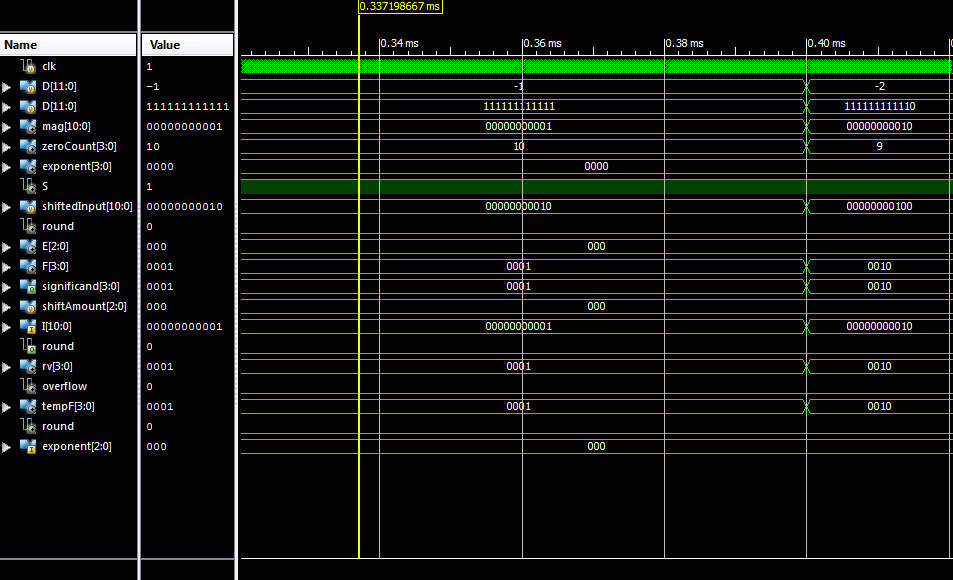
\includegraphics[width=10cm]{waveform.PNG}

\lstinputlisting[language=Verilog, firstline=1, lastline=2]{fpcvt.v}

\lstinputlisting[language=Verilog, firstline=25, lastline=26]{tb.v}

\end{document}

